\section{Entropy}

Symmetric functions $H_m\left(p_1, p_2, \ldots, p_m\right)$ 满足以下条件: \\
1. Normalization: $H_2\left(\dfrac{1}{2}, \dfrac{1}{2}\right)=1$ \\
2. Continuity: $H_2(p, 1-p)$ is a continuous function of $p$ \\
3. Grouping: $H_m\left(p_1, p_2, \ldots, p_m\right)=H_{m-1}\left(p_1+p_2, p_3, \ldots, p_m\right)+\left(p_1+p_2\right) H_2\left(\dfrac{p_1}{p_1+p_2}, \dfrac{p_2}{p_1+p_2}\right)$ \\
具有如下图所示的拆分/合并性质:
\begin{figure}[htbp]
    \centering
    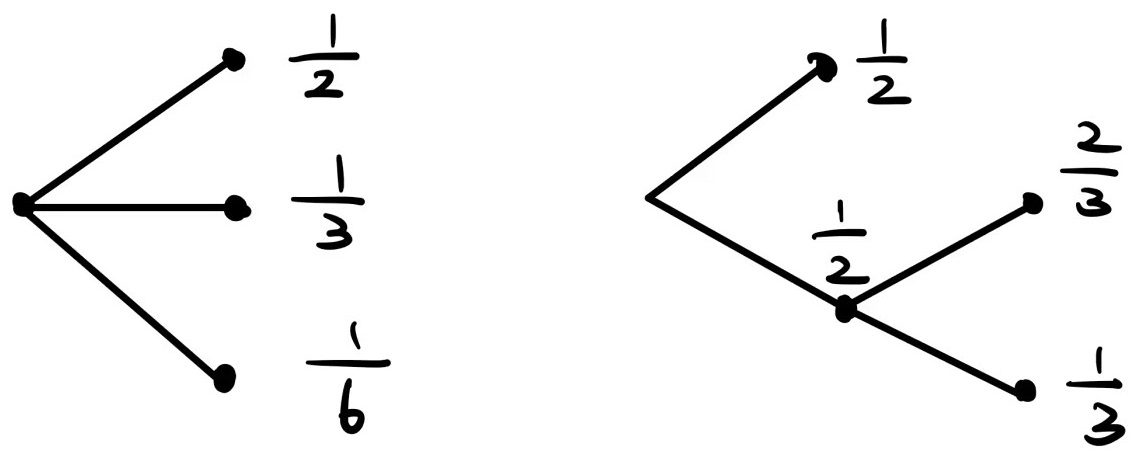
\includegraphics[width=0.6\textwidth]{./figures/chapter1/entropy_deduction.png}
\end{figure}
$$H(X)=H\left(\dfrac{1}{2},\dfrac{1}{3},\dfrac{1}{6}\right)=H\left(\dfrac{1}{2},\dfrac{1}{2}\right)+\dfrac{1}{2}H\left(\dfrac{2}{3},\dfrac{1}{3}\right)$$

具体简要推导见Appendix \ref{sec:Axiomatic_definition_of_entropy}, 最后能够推导出$H(X)$的唯一形式为
$$H(X)=k\cdot \sum_{x\in\mathcal{X}}p(x)\log\dfrac{1}{p(x)}$$

\begin{definition}
事件$x$发生的概率为$p(x)$, 则$x$的信息量为$\log\dfrac{1}{p(x)}$.
\end{definition}

\begin{definition}
离散型随机变量$X$的熵 (entropy) $H(X)$:
\begin{align*}
    H(X)&= -\sum_{x\in\mathcal{X}}p(x)\log p(x) \\
        &= \sum_{x\in\mathcal{X}}p(x)\log\dfrac{1}{p(x)} \\
        &= \mathbb{E}\left[\log\dfrac{1}{p(x)}\right]
\end{align*}
\end{definition}

$H(X)$物理意义: $X=x$ 事件发生的概率$p(x)$, 信息量为 $\log\dfrac{1}{p(x)}$. \\
$H(X)$: 所有事件发生的期望信息量.

\begin{proposition}
$H(X)\geq 0$, 当且仅当$p(x)=1$时, $H(X)=0$.\\
$p(x)=1$时, 事件是确定的(deterministic), 信息量为0.
\end{proposition}

\begin{definition}
$X\in \mathcal{X}, Y\in\mathcal{Y}; |\mathcal{X}|,|\mathcal{Y}|<\infty$(离散型随机变量). \\
$X$和$Y$的联合熵 (joint entropy) $H(X,Y)$:
\begin{align*}
    H(X,Y)&= -\sum_{x\in\mathcal{X}}\sum_{y\in\mathcal{Y}}p(x,y)\log p(x,y) \\
        &= \sum_{x\in\mathcal{X}}\sum_{y\in\mathcal{Y}}p(x,y)\log\dfrac{1}{p(x,y)} \\
        &= \mathbb{E}\left[\log\dfrac{1}{p(x,y)}\right]
\end{align*}
\end{definition}

\begin{proposition}
$0\leq H(X)\leq \log|\mathcal{X}|$.\\
$X$为冲激函数时取$0$ (deterministic), $X$为均匀分布时取$\log|\mathcal{X}|$.\\
prove 均匀分布时取得最大值 $\log|\mathcal{X}|$:\\
Let $u(x)=\dfrac{1}{|\mathcal{X}|}$, then
\begin{align*}
D\left(p\|u\right) &= \sum_{x\in\mathcal{X}}p(x)\log\dfrac{p(x)}{u(x)} \\
&= \sum_{x\in\mathcal{X}}p(x)\log|\mathcal{X}| - \sum_{x\in\mathcal{X}}p(x)\log\dfrac{1}{p(x)} \\
&= \log|\mathcal{X}| - H(X) \\
&\geq 0
\end{align*}
当且仅当$p(x)=u(x)$时等号成立, i.e. $H(X)$取得最大值 $\log|\mathcal{X}|$.
\end{proposition}


\begin{definition}
条件熵 (conditional entropy) $H(Y|X)$:
\begin{align*}
    H(Y|X)&= \textcolor{red}{\sum_{x\in\mathcal{X}}p(x)H(Y|X=x)} \\
        &= -\sum_{x\in\mathcal{X}}p(x)\sum_{y\in\mathcal{Y}}p(y|x)\log p(y|x) \\
        &= \textcolor{red}{\sum_{x\in\mathcal{X}}\sum_{y\in\mathcal{Y}}p(x,y)\log\dfrac{1}{p(y|x)}} \\
        &= \mathbb{E}\left[\log\dfrac{1}{p(y|x)}\right]
\end{align*}
\end{definition}

\begin{theorem}
    chain rule 剥洋葱:
    $$H(X,Y)=H(X)+H(Y|X)$$
\end{theorem}


\begin{example}
Find $H(X), H(Y), H(X|Y), H(X,Y)$.
\begin{table*}[!htbp]
    \centering
    \begin{tabular}{|c|c|c|c|c|}
        \hline \diagbox{$Y$}{$X$} & $1$ & $2$ & $3$ & $4$  \\
        \hline $1$ & $\frac{1}{8}$ & $\frac{1}{16}$ & $\frac{1}{32}$ & $\frac{1}{32}$ \\
        \hline $2$ & $\frac{1}{32}$ & $\frac{1}{32}$ & $\frac{1}{32}$ & $\frac{1}{32}$ \\
        \hline $3$ & $\frac{1}{16}$ & $\frac{1}{16}$ & $\frac{1}{16}$ & $\frac{1}{16}$ \\
        \hline $4$ & $\frac{1}{4}$  & 0 & 0 & 0 \\
        \hline
    \end{tabular}
\end{table*}

$$H(X)=H\left(\dfrac{1}{2},\dfrac{1}{4},\dfrac{1}{8},\dfrac{1}{8}\right)=\dfrac{7}{4}\text{bits}$$
$$H(Y)=H\left(\dfrac{1}{4},\dfrac{1}{4},\dfrac{1}{4},\dfrac{1}{4}\right)=\log 4 = 2\text{bits} \ (\textcolor{red}{uniform\ distribution})$$
\begin{align*}
H(X|Y)&= \sum_{y\in\mathcal{Y}}p(y)H(X|Y=y) \\
    &= \dfrac{1}{4}\left(H\left(\dfrac{1}{2},\dfrac{1}{4},\dfrac{1}{8},\dfrac{1}{8}\right)+H\left(\dfrac{1}{4},\dfrac{1}{2},\dfrac{1}{8},\dfrac{1}{8}\right)+H\left(\dfrac{1}{4},\dfrac{1}{4},\dfrac{1}{4},\dfrac{1}{4}\right)+H\left(1\right)\right) \\
    &= \dfrac{11}{8} \text{bits}
\end{align*}
$H(X,Y)=H(Y)+H(X|Y)=2+\dfrac{11}{8}=\dfrac{27}{8}$ bits.
\end{example}

\begin{proposition}
\begin{align*}
    H(X,Y) &= H(X) + H(Y) \text{\ \ \ ($X\perp Y$)} \\
    H(X,Y) &= H(X) \text{\ \ \ \ \ \ \ \ \ \ \ \ \ \ ($Y=X$)}
\end{align*}
\end{proposition}